\documentclass[12pt,a4paper]{article}
\usepackage{cmap} % Makes the PDF copiable. See http://tex.stackexchange.com/a/64198/25761
\usepackage[T1]{fontenc}
\usepackage[brazil]{babel}
\usepackage[utf8]{inputenc}
\usepackage{amsmath}
\usepackage{amsfonts}
\usepackage{amssymb}
\usepackage{amsthm}
\usepackage{textcomp} % \degree
\usepackage{gensymb} % \degree
\usepackage[usenames,svgnames,dvipsnames]{xcolor}
\usepackage{hyperref}
\usepackage{multicol}
\usepackage{graphicx}
\usepackage[margin=2cm]{geometry}
\usepackage{systeme}
\usepackage{cancel}

\hypersetup{
    colorlinks = true,
    allcolors = {blue}
}

% TODO: Consider using exsheets
% http://linorg.usp.br/CTAN/macros/latex/contrib/exsheets/exsheets_en.pdf
%
% http://ctan.org/tex-archive/macros/latex/contrib/exercise/
% Options: answerdelayed,lastexercise,noanswer
\usepackage[answerdelayed,lastexercise]{exercise}

\addto\captionsbrazil{%
\def\listexercisename{Lista de exerc\'icios}%
\def\ExerciseName{Exerc\'icio}%
\def\AnswerName{Solu\c{c}\~ao do exerc\'icio}%
\def\ExerciseListName{Ex.}%
\def\AnswerListName{Solu\c{c}\~ao}%
\def\ExePartName{Parte}%
\def\ArticleOf{de\ }%
}

\renewcommand{\ExerciseHeaderTitle}{(\ExerciseTitle)\ }
\renewcommand{\ExerciseListHeader}{%\ExerciseHeaderDifficulty%
\textbf{%\ExerciseListName\
\ExerciseHeaderNB.\ %
%\ --- \
\ExerciseHeaderTitle}%
%\ExerciseHeaderOrigin
\ignorespaces}
\renewcommand{\AnswerListHeader}{\textbf{\ExerciseHeaderNB.\ (\AnswerListName)\ }}

\renewcommand{\theenumi}{\alph{enumi}}
\renewcommand\labelenumi{(\theenumi) }

\newcommand*\tipo{Prova III}
\newcommand*\turma{PRO112-04U}
\newcommand*\disciplina{CAN0001}
\newcommand*\eu{Helder G. G. de Lima}
\newcommand*\data{28/11/2017}

\author{\eu}
\title{\tipo - \disciplina}
\date{\data}

\begin{document}
\thispagestyle{empty}
\newgeometry{margin=2cm,bottom=0.5cm}
\begin{center}

\includegraphics[width=9.0cm]{marca} \\
\textbf{\tipo\ (\disciplina / \turma)} \\
Prof. \eu\footnote{
Este é um material de acesso livre distribuído sob os termos da licença \href{https://creativecommons.org/licenses/by-sa/4.0/deed.pt_BR}{Creative Commons Atribuição-CompartilhaIgual 4.0 Internacional}}
\end{center}

\noindent Nome do(a) aluno(a): \underline{\hspace{9,7cm}} Data: \underline{\data}

%\section*{Instruções}
\begin{center}\fbox{
\begin{minipage}{15cm}

{\footnotesize
\begin{itemize}
\renewcommand{\theenumi}{\Roman{enumi}}
\item Identifique-se em todas as folhas.
\item Mantenha o celular e os demais equipamentos eletrônicos desligados durante a prova.
\item Justifique cada resposta com cálculos ou argumentos baseados na teoria estudada.
\item Utilize números decimais em vez de frações e arredonde-os com 4 casas depois da vírgula.
\item Resolva apenas os itens de que precisar para somar 10,0 pontos.
\end{itemize}
}

\end{minipage}
}
\end{center}

%\section*{Questões}
\begin{ExerciseList}
\Exercise[title={2,5}]
A figura a seguir representa um lago, e inclui as coordenadas (em metros) de alguns pontos de sua margem. Estime a área do lago por meio da repetição da regra 3/8 de Simpson no máximo de intervalos que for possível.
\begin{center}
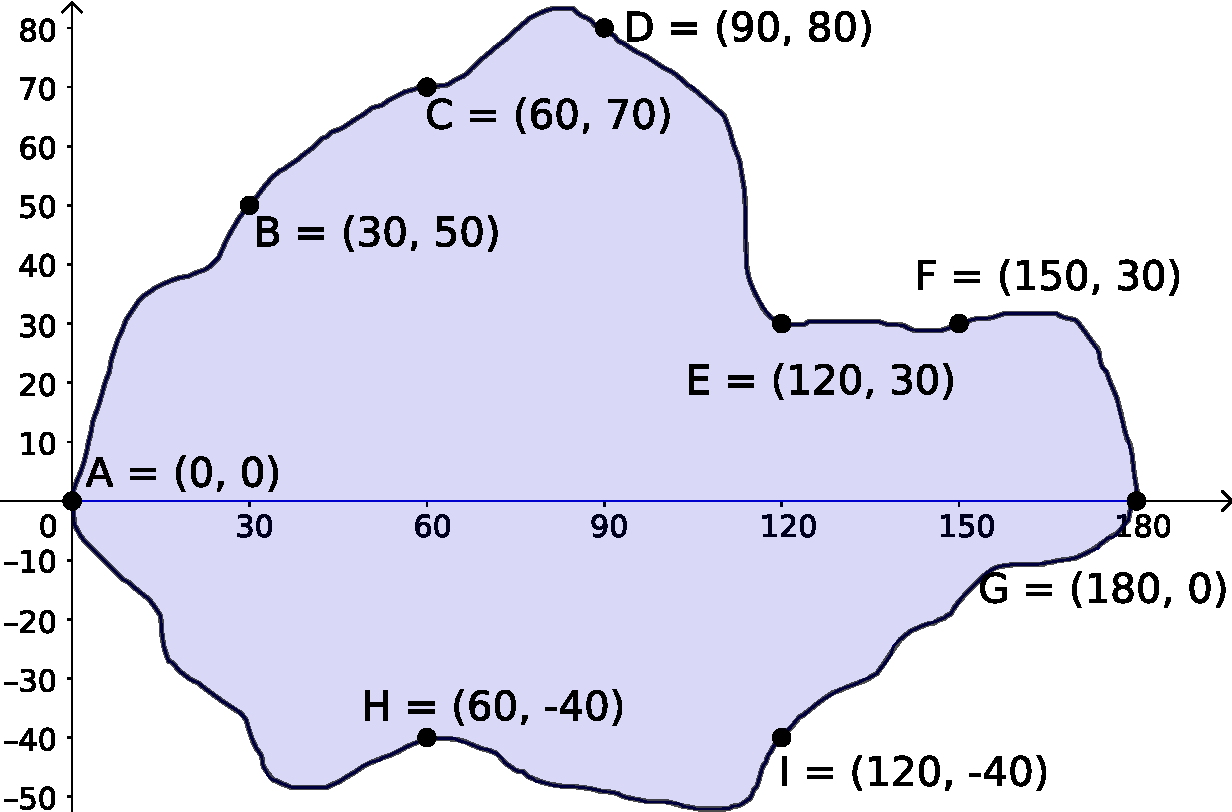
\includegraphics[height=7.0cm]{img/prova-3-pro-1-lago.pdf}
\end{center}
\Answer Considerando a margem superior do lago como sendo o gráfico de uma função $f$, e a margem inferior o gráfico de $g$, pode-se determinar a área do lago calculando a soma das áreas (que são positivas) entre o eixo horizontal e cada uma das funções, isto é:
\begin{align*}
A & = \int_0^{180} |f(x)| dx + \int_0^{180} |g(x)| dx
    = \left( \int_0^{90} |f(x)| dx + \int_{90}^{180} |f(x)| dx \right)
    + \int_0^{180} |g(x)| dx\\
  & \approx
  \underbrace{
    \frac{3}{8} \cdot 30 \cdot (0 +3\cdot 50 +3\cdot 70+80)
  + \frac{3}{8} \cdot 30 \cdot (80+3\cdot 30 +3\cdot 30+ 0)
  }_{\text{Área aproximada da parte superior}}\\
& + \underbrace{
  \frac{3}{8} \cdot 60 \cdot
  (0+3\cdot |-40|+3\cdot |-40|+0)
  }_{\text{Área aproximada da parte inferior}}\\
&=  \frac{90}{8} \cdot 440 + \frac{180}{8}\cdot 260
 = 7875+5400 = 13275 m^2
\end{align*}
As aproximações acima correspondem à interpolação dos dados por meio de 3 funções de grau menor ou igual a 3, como na figura a seguir:
\begin{center}
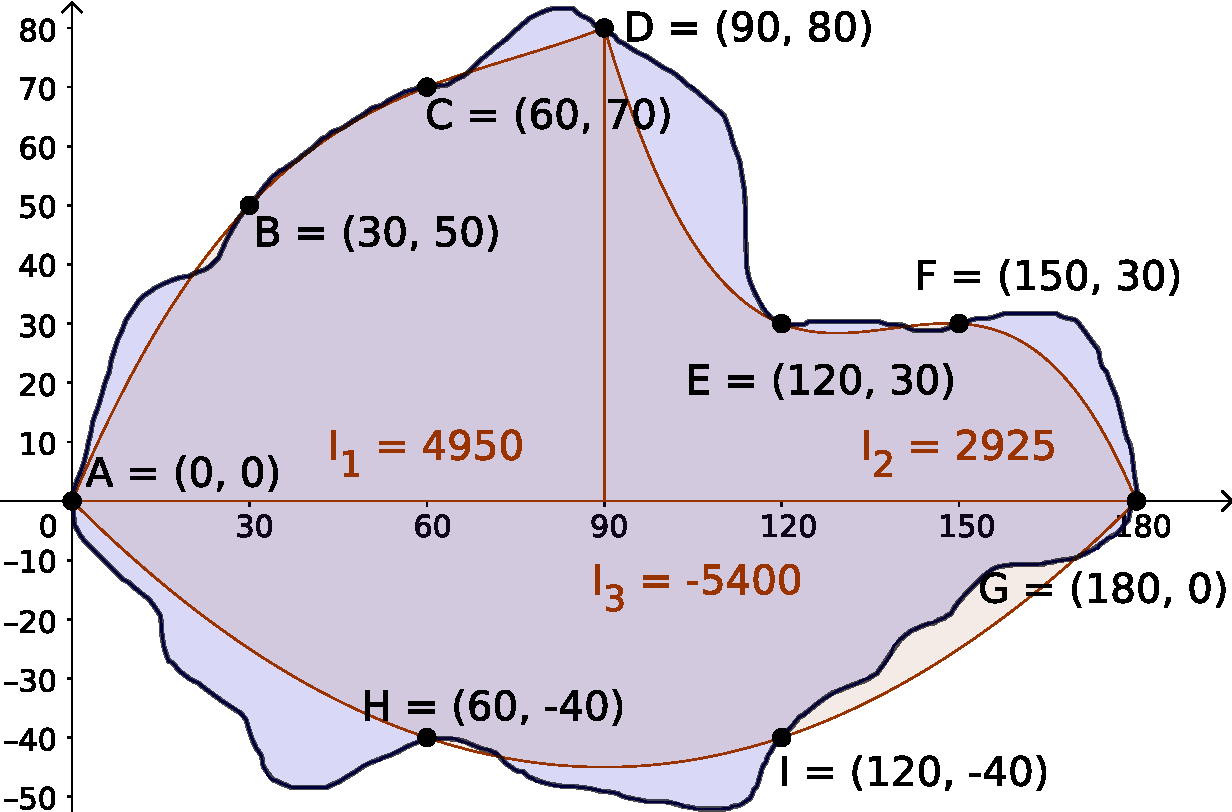
\includegraphics[height=5.0cm]{img/prova-3-pro-1-lago-aprox.pdf}
\end{center}

\Exercise[title={2,5}]
Verifique se ao estimar $\displaystyle I = \int_0^2 2^x\ dx = 3/\ln(2)$ usando a regra de Gauss-Legendre com 4 pontos o resultado é mais preciso do que com 5 pontos. \textit{\footnotesize (Use 4 dígitos após a vírgula)}
\Answer
Fazendo a mudança de variáveis $x = t + 1$, tem-se $dx = dt$ e
$\int_0^2 2^x dx = \int_{-1}^1 2^{t+1} dt$.
Assim, pode-se aplicar o método de Gauss-Legendre, arredondando todos os valores relevantes com 4 dígitos após a vírgula, para obter:
\begin{itemize}
\item Com 4 pontos:
\begin{align*}
I & \approx
  0.347\textbf{9} \cdot 2^{(-0.8611 + 1)}
+ 0.6521 \cdot 2^{(-0.3\textbf{400} + 1)}
+ 0.6521 \cdot 2^{( 0.3\textbf{400} + 1)}
+ 0.347\textbf{9} \cdot 2^{( 0.8611 + 1)}\\
& =
  0.3479 \cdot 1.1011
+ 0.6521 \cdot 1.5801
+ 0.6521 \cdot 2.5315
+ 0.3479 \cdot 3.6328\\
& = 0.3831 + 1.0304 + 1.6508 + 1.2639 = 4.3282
\end{align*}
\item Com 5 pontos:
\begin{align*}
I & \approx
  0.2369 \cdot 2^{(-0.906\textbf{2} + 1)}
+ 0.4786 \cdot 2^{(-0.538\textbf{5} + 1)}
+ 0.568\textbf{9} \cdot 2^1
+ 0.4786 \cdot 2^{( 0.538\textbf{5} + 1)}
+ 0.2369 \cdot 2^{( 0.906\textbf{2} + 1)}\\
&=
  0.2369 \cdot 1.0672
+ 0.4786 \cdot 1.3770
+ 0.5689 \cdot 2
+ 0.4786 \cdot 2.9049
+ 0.2369 \cdot 3.7482\\
&= 0.2528 + 0.6590 + 1.1378 + 1.3903 + 0.8879 = 4.3278
\end{align*}
\end{itemize}
Como $3/\ln(2) = 4,3281$, então os módulos dos erros absolutos são $\varepsilon_4 = 0.0001 < 0.0003 = \varepsilon_5$. Por outro lado, os erros relativos são $\varepsilon_{per,4} = 0.0000231 < 0.00006932 = \varepsilon_{per,5}$.

\Exercise[title={2,5}]
Aplique o método de Romberg para estimar $\int_{-1}^3 \sqrt[3]{x}\ dx \approx R_{k,k}$ com um erro relativo percentual de no máximo 0.02\%. O valor exato é $2.495061533\ldots$ \textit{\footnotesize(Use 4 dígitos após a vírgula)}
\Answer
Para que a estimativa $R_{k,k}$ tenha um erro de no máximo $0.02\%$ em relação ao valor exato $I$, ela deve estar no intervalo $(I-0.02\%, I+0.02\%) = (\mathbf{2.49}46, \mathbf{2.49}56)$. Calculando os termos $R_{k,j}$, obtêm-se:
\begin{multicols}{2}
\begin{itemize}
\item $R_{1,1}
= \frac{4}{2}(-1 + \sqrt[3]{3})
= 0.8845$
\item $R_{2,1}
= \frac{4}{4}(-1 + 2\sqrt[3]{1} + \sqrt[3]{3})
= 2.4422$
\item $R_{2,2}
= 2.4422+\frac{2.4422-0.8845}{3}
= 2.9614$
\item $R_{3,1}
= \frac{4}{8}(-1 + 2(0 + 1 + \sqrt[3]{2}) + \sqrt[3]{3})\\
= 2.4810$
\item $R_{3,2}
= 2.4810+\frac{2.4810-2.4422}{3}
= 2.4939$
\item $R_{3,3}
= 2.4939+\frac{2.4939-2.9614}{15}
= 2.4627$
\item $R_{4,1}
= \frac{4}{8}(-1 + 2(\cancel{ \sqrt[3]{-0.5} } + 0 + \cancel{ \sqrt[3]{0.5} } + 1 + \sqrt[3]{1.5} + \sqrt[3]{2}) + \sqrt[3]{3})
= 2.4915$
\item $R_{4,2}
= 2.4915+\frac{2.4915-2.4810}{3}
= 2.4950$
\item $R_{4,3}
= 2.4950+\frac{2.4950-2.4939}{15}
= 2.4951$
\item $R_{4,4}
= 2.4951+\frac{2.4951-2.4627}{63}
= 2.4956$
\end{itemize}
\end{multicols}

Os resultados anteriores são resumidos na tabela a seguir, juntamente com os erros relativos percentuais correspondentes aos termos $R_{k,k}$:
\begin{center}
\begin{tabular}{|c|c|c|c|c|r|}
\hline
$\mathbf{k}$ & $\mathbf{ R_{k,1} }$ & $\mathbf{ R_{k,2} }$ & $\mathbf{ R_{k,3} }$ & $\mathbf{ R_{k,4} }$ & \textbf{Erro \%} \\
\hline
1& \textbf{0,8845} &  &  &  & -64,55\% \\
\hline
2& 2,4422 & \textbf{2,9614} & & & 18,69\% \\
\hline
3& 2,4810 & 2,4939 & \textbf{2,4627} & & -1,30\% \\
\hline
4& 2,4915 & 2,4950 & 2,4951 & \textbf{2,4956} & 0,02\% \\
\hline
\end{tabular}
\end{center}

\Exercise%[title={2,5}]
Considere a equação diferencial $y^\prime(t) = y(t) - t$.
\begin{enumerate}
\item \textbf{(2,5)} Use os métodos de Euler explícito e implícito para estimar $y(t)$ conforme $t$ percorre o intervalo $[1, 2]$ com passos de tamanho $h = 0.25$, dada a condição inicial $y(1) = 2$. Comente os resultados obtidos, levando em conta que a solução exata é $y(t)=t+1$.
\item \textbf{(2,5)} Use os métodos de Runge-Kutta de ordem 2 e 4 para estimar $y(t)$ conforme $t$ percorre o intervalo $[0, 3]$ com passos de tamanho $h = 1$, dada a condição inicial $y(0) = 0.8$. Comente os resultados obtidos, levando em conta que a solução exata é $y(t)=t+1-0.2e^t$.
\end{enumerate}
\Answer
\begin{enumerate}
\item Denotando $f(t,y) = y-t$ e $h=0.25$, pode-se expressar a fórmula do método de Euler explícito da seguinte forma:
\[
y_{i+1}
= y_i + h f(t_i, y_i)
= y_i + 0.25( y_i - t_i )
= 1.25 y_i - 0.25 t_i.
\]
Disto resulta que os valores obtidos a cada passo são os seguintes:
\begin{center}
\begin{tabular}{|c|c|r|c|c|}
\hline
$i$ & $t_i$ & $y_i= 1.25 y_{i-1} - 0.25 t_{i-1}$ & $y_{exato}(t_i)$ & $\varepsilon_i = y_i-y_{exato}(t_i)$ \\ \hline\hline
$0$ & $1.00$ & $2.00$ & $2.00$ & $0.00$ \\ \hline
$1$ & $1.25$ & $1.25 \cdot 2.00 - 0.25 \cdot 1.00 = 2.25$ & $2.25$ & $0.00$ \\ \hline
$2$ & $1.50$ & $1.25 \cdot 2.25 - 0.25 \cdot 1.25= 2.50$ & $2.50$ & $0.00$ \\ \hline
$3$ & $1.75$ & $1.25 \cdot 2.50 - 0.25 \cdot 1.50 = 2.75$ & $2.75$ & $0.00$ \\ \hline
$4$ & $2.00$ & $1.25 \cdot 2.75 - 0.25 \cdot 1.75 = 3.00$ & $3.00$ & $0.00$ \\ \hline
\end{tabular}
\end{center}
No método de Euler implícito, por sua vez, utiliza-se a relação $y_{i+1} = y_i + h f(t_{i+1}, y_{i+1})$ que, no problema considerado, pode ser reescrita  de forma equivalente como:
\[
y_{i+1}
= y_i + \frac{1}{4}( y_{i+1} - t_{i+1} )
\Leftrightarrow
4y_{i+1} = 4y_i + y_{i+1} - t_{i+1}
\Leftrightarrow
y_{i+1} = (4y_i-t_{i+1})/3.
\]
Consequentemente, os valores obtidos a cada passo são:
\begin{center}
\begin{tabular}{|c|c|r|c|c|}
\hline
$i$ & $t_i$ & $y_{i+1} = (4y_i-t_{i+1})/3$ & $y_{exato}(t_i)$ & $\varepsilon_i = y_i-y_{exato}(t_i)$ \\ \hline\hline
$0$ & $1.00$ & $2.00$ & $2.00$ & $0.00$ \\ \hline
$1$ & $1.25$ & $(4 \cdot 2.00-1.25)/3 = 2.25$ & $2.25$ & $0.00$ \\ \hline
$2$ & $1.50$ & $(4 \cdot 2.25-1.50)/3 = 2.50$ & $2.50$ & $0.00$ \\ \hline
$3$ & $1.75$ & $(4 \cdot 2.50-1.75)/3 = 2.75$ & $2.75$ & $0.00$ \\ \hline
$4$ & $2.00$ & $(4 \cdot 2.75-2.00)/3 = 3.00$ & $3.00$ & $0.00$ \\ \hline
\end{tabular}
\end{center}
No problema considerado, ambas as versões do método de Euler fornecem valores exatos ao longo de todo o intervalo. Isso já era esperado, uma vez que os métodos de Euler são baseados na aproximação da solução por meio de pequenos segmentos de reta, e a solução exata do problema dado é uma função afim. A ausência de curvatura na solução exata impede que ocorra qualquer erro ao aproximá-la por retas tangentes (pois são coincidentes).

\item Pelo método de Runge-Kutta de ordem 2, obtêm-se:
\begin{center}
\begin{tabular}{|c|c|r|r|c|r|c|}
\hline
  $i$
& $t_i$
& $k_1$
& $k_2$
& $y_i$
& $y_{exato}(t_i)$
& $\varepsilon_i = y_i-y_{exato}(t_i)$ \\ \hline\hline
$0$ & $0.00$ &   -     &   -     & $ 0.800$ & $ 0.8000$ & $0.0000$ \\ \hline
$1$ & $1.00$ & $ 0.80$ & $ 0.06$ & $ 1.500$ & $ 1.4563$ & $0.0437$ \\ \hline
$2$ & $2.00$ & $ 0.50$ & $ 0.00$ & $ 1.750$ & $ 1.5222$ & $0.2278$ \\ \hline
$3$ & $3.00$ & $-0.25$ & $-1.50$ & $ 0.875$ & $-0.0171$ & $0.8921$ \\ \hline
\end{tabular}
\end{center}

Já pelo método de Runge-Kutta de ordem 4, obtêm-se:
\begin{center}
\begin{tabular}{|c|c|r|r|r|r|c|r|c|}
\hline
  $i$
& $t_i$
& $k_1$
& $k_2$
& $k_3$
& $k_4$
& $y_i$
& $y_{exato}(t_i)$
& $\varepsilon_i = y_i-y_{exato}(t_i)$ \\ \hline\hline
$0$ & $0.00$ &   -     &   -     &   -     &   -     & $ 0.8000$ & $ 0.8000$ & $0.0000$ \\ \hline
$1$ & $1.00$ & $ 0.8000$ & $ 0.7000$ & $ 0.6500$ & $ 0.4500$ & $ 1.4583$ & $ 1.4563$ & $0.0020$ \\ \hline
$2$ & $2.00$ & $ 0.4583$ & $ 0.1875$ & $ 0.0521$ & $-0.4896$ & $ 1.5330$ & $ 1.5222$ & $0.0108$ \\ \hline
$3$ & $3.00$ & $-0.4670$ & $-1.2005$ & $-1.5673$ & $-3.0343$ & $ 0.0268$ & $-0.0171$ & $0.0439$ \\ \hline
\end{tabular}
\end{center}
Pode-se observar que, embora o método de ordem 4 exija mais 2 avaliações da função a cada passo, ele permite uma redução significativa dos erros absolutos ao longo do intervalo, sem a necessidade de reduzir o tamanho do passo (ou, o que seria equivalente, aumentar o número de passos dados).

\end{enumerate}
\end{ExerciseList}

\vspace{0.4cm}
\begin{center}
BOA PROVA!
\end{center}

\newpage
\restoregeometry
\section*{Respostas}
\shipoutAnswer
\end{document}
